\documentclass[tikz,border=3pt]{standalone}
\usepackage[utf8]{inputenc}
\usepackage[T1]{fontenc}
\usepackage{lmodern}
\renewcommand{\familydefault}{\sfdefault}
\usepackage{sansmath}\sansmath
\usepackage{chemfig}
\usepackage{pgfplots}\pgfplotsset{compat=1.18,/pgf/number format/use comma,/pgf/number format/1000 sep={.}}
\usetikzlibrary{arrows.meta,calc,positioning,decorations.pathmorphing,patterns}
% paleta del sitio
\definecolor{nar}{HTML}{E8680C}\definecolor{narc}{HTML}{FFB35C}\definecolor{hielo}{HTML}{FFF3E8}
\definecolor{tinta}{HTML}{1D1D1F}\definecolor{gris}{HTML}{6E6E73}\definecolor{lila}{HTML}{7C5CF0}
\definecolor{azul}{HTML}{2F6FD6}\definecolor{menta}{HTML}{17A673}\definecolor{coral}{HTML}{E8342A}
\tikzset{cel/.style={draw=gris,fill=hielo,line width=0.9pt},nuc/.style={draw=gris!70,line width=0.6pt},
fib/.style={gris!55,line width=0.35pt},eti/.style={font=\footnotesize,text=tinta,align=center},
num/.style={circle,draw=nar,fill=white,text=nar,font=\small\bfseries,inner sep=1.2pt,minimum size=13pt},
fl/.style={-{Stealth[length=2.6mm]},gris,line width=0.9pt}}
\begin{document}
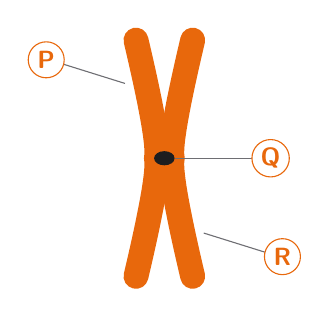
\begin{tikzpicture}[font=\small]
\draw[nar,line width=9pt,line cap=round] (-0.36,1.5) .. controls (-0.1,0.4) and (-0.08,0.1) .. (-0.1,0) .. controls (-0.08,-0.1) and (-0.1,-0.4) .. (-0.36,-1.5);
\draw[nar,line width=9pt,line cap=round] (0.36,1.5) .. controls (0.1,0.4) and (0.08,0.1) .. (0.1,0) .. controls (0.08,-0.1) and (0.1,-0.4) .. (0.36,-1.5);
\fill[tinta] (0,0) ellipse (0.13 and 0.09);
\draw[gris] (-0.5,0.95)--(-1.3,1.2);\node[num] at (-1.5,1.25) {P};
\draw[gris] (0.13,0)--(1.15,0);\node[num] at (1.35,0) {Q};
\draw[gris] (0.5,-0.95)--(1.3,-1.2);\node[num] at (1.5,-1.25) {R};
\end{tikzpicture}
\end{document}
